%%%%%%%%%%%%%%%%%%%%%%%%%%
% Edited by Rachel Grotheer, Wofford College from
% A template for Technical Report
% Prof. Siraj Shaikh
% Dr. Hoang Nga Nguyen
% Coventry University
% 2020
%%%%%%%%%%%%%%%%%%%%%%%%%%


\documentclass[12pt]{article}
\usepackage[margin=1.2in]{geometry}
\usepackage[toc,page]{appendix}
\usepackage{graphicx}
\usepackage[square,numbers]{natbib}
\usepackage{lipsum}
\usepackage{caption}
\usepackage{pdfpages}
\usepackage{amsmath}

\begin{document}

\captionsetup[figure]{margin=1.5cm,font=small,labelfont={bf},name={Figure},labelsep=colon,textfont={it}}
\captionsetup[table]{margin=1.5cm,font=small,labelfont={bf},name={Table},labelsep=colon,textfont={it}}
\SetLipsumDefault{1}


\begin{center}
\thispagestyle{empty}
{\LARGE Wofford College}\\[.5cm]
{\Large Department of Mathematics}\\[3cm]
{\linespread{1.2} {\Large Technical Report}}\\[0.5cm]
{\huge \bfseries Maximizing Accessibility in Spartanburg's Bus Sytem}\\[1.5cm]
\linespread{1}

\includegraphics[width=3.5cm]{images/Woff_logo.png}\\[1cm]
\vspace{\fill}
{\Large Authors: Townshend Gillespie, Caroline Kirk, Aidan Langston-Smith, Ryan Methot, Juan Salas}

{\Large \today}
\end{center}

\clearpage
\pagenumbering{arabic}

% -------------------------------------------------------------------
% Contents, list of figures, list of tables
% -------------------------------------------------------------------
\section*{Executive Summary}

This paper is an analysis of the accessibility to services and amenities of Spartanburg's bus routes.  The city of Spartanburg, SC is growing and is home to many companies headquarters including Denny's and Milliken.  Since Spartanburg is a growing city, it is important to look at the public transportation and see how accessible it is for the average community member.  We examined a few bus stops on multiple bus routes in Spartanburg, SC and determined whether or not the bus stops were "good" based on their relative distance to different amenities.  Looking at existing maps of Spartanburg bus stops, we created a 0.6 mile radius around different stops and looked at what amenities were within the radius.  The 0.6 mile radius was used in assumption that the average person is willing to walk that far to reach any service or amenity.  

Another important assumption we had to make was the importance of our selected services and amenities.  We assumed importance based off of how many times someone would go to that particular amenity and then gave them a point value between 1 and 10.  For example, a grocery store is visited on average once a week, so it has the highest score of 10.  Once we had our point system organized, we created our model which is an equation that takes into consideration the assigned point values of different amenities, as well as the number of amenities that are in the 0.6 mile radius.  By solving the model, it gives a point value that can be used to determine if a bus stop is "good". 

One important limitation that we have in regard to this model is the lack of community input.  Based off of time constraints, there was not opportunity to interview community members to see how often people are using the bus system, where they are going, or where they need  to go. This model is based off of our assumptions of how amenities rank in importance, which is variable among people.  We also did not take into consideration how bus stops are located among different residential areas.

Using our full model analysis, we came to the conclusion that the Dorman Center Inbound Stop 2 is considered to be a good stop with an accessibility score of 74.  However, the South Liberty Inbound stop is considered to be a bad stop with an accessibility score of 36.  We observed multiple stops with varying different accessibility scores indicating that the bus routes in Spartanburg have different levels of accessibility.
\newpage
\tableofcontents
%\listoffigures
%\listoftables

\newpage

% -------------------------------------------------------------------
% Main sections (as required)
% -------------------------------------------------------------------

\section{Introduction}

\subsection{Problem Overview}

Spartanburg is a growing city in the Upstate region of South Carolina that is home to the headquarters of multiple reputable companies, such as Denny's and Milliken. As a city grows in population, its infrastructure needs to grow simultaneously in order to maintain a stable environment for both residents and industries. Public transportation is an aspect of city infrastructure that has become increasingly important in urban centers everywhere.  While Spartanburg has strong foundations in this area, improvements can be made. We were tasked with making improvements by determining a method to maximize accessibility to public services and amenities in Spartanburg through the means of the bus system. 

\subsection{Aims and Objectives}

As previously stated, the main objective of our model was to develop a method to maximize accessibility to services and amenities through the public bus system in Spartanburg, South Carolina. In order to do this, we sought to create something that can serve as a means of assessing accessibility for both existing stops and locations for potential new stops. Considering this, we came up with the following problem statement:
\linebreak
\linebreak
    \textit{Our model will predict the optimal places to put bus stops in Spartanburg by finding areas that would maximize the amount of reachable and important services and amenities.}

\subsection{Overview Statistics}

This is a problem with minimal existing research and data that are specific to the city of Spartanburg. However, we do have some insightful statistics on the infrastructure and residents of Spartanburg. After manually collecting data on all of the services and amenities within Spartanburg that fall into various categories (Appendix A), we can see that there are 16 pharmacies, 39 grocery stores, 15 laundromats, and 21 medical facilities available within the city. To put those numbers in context, the 2022 United States Census reports that there are 38,584 residents in the city of Spartanburg. This shows that there are plenty of valuable services and amenities available to the residents in Spartanburg that can accessed through the bus routes.
\linebreak
\linebreak
In addition to this data, we were also able to find data collected by the U.S. Census Bureau in 2022 that showed various statistics about employed workers in Spartanburg County (Appendix B). In this dataset, it shows the amount of vehicles that workers reported as being available to them, as well as showing the means of transportation that workers reported using in order to get to their jobs. After performing a simple data summary (Appendix C), we found that an estimated 20.8 percent of workers in the Spartanburg area have 1 or less cars available to them, which shows that a large portion of residents could realistically benefit from improved public transportation. Additionally, we found that the vast majority of workers that claimed to walk to work also reported having no vehicle available to them. This could indicate that the current bus system does not reach the employers of many residents in the area who are in critical need of efficient public transport due to a lack of personal vehicles. We feel that these statistics are good motivators for the problem we are seeking to solve, as they show the legitimate need from the community for an improved bus system.


\section{Model and Solution}


\subsection{Assumptions}

    We have made a prioritized list of the different categories of services/amenities in the city to more accurately assess how a stop would be “good” in terms of maximizing access to those services. This in itself is a big assumption that we have mostly created based on intuition, but plan to revise and back up based on articles and data that we find. This is what the priority list looks like so far:


Groceries (1 day a week),
Pharmacies ( 1 day a month),
Medical Facility (irregular but important visits),
Religious Buildings (1 day a week),
Laundromats (1 day a week),
Retail Stores (1 day a week),
Community centers (1-3 days a week, recreational), and
Restaurants (1-2 days a week) (Table 1).



Our estimates of how often a service is visited (and potentially how important those visits are) are a big part of how we made this list. Overall, we feel that the top three:  grocery stores, pharmacies, and medical facilities are  the most important because of how essential they are to anyone’s life. The next three are potentially essential to someone’s life based on their circumstances and/or lifestyle. Then, the last three are places that are still important and regularly visited, but not necessarily essential by any means.

The model has been constructed under the assumption that bus riders will be willing to walk for a time of at most 15 minutes to get to a bus stop, and/or get to services within 15 minutes walk from a bus stop.  The average adult human over 60 years walks at a speed of 1.21 meters/sec (Alves et al., 2020) hence if we calculate the maximum distance to and from a bus stop we get:

\[(1.21\text{ meters/s})(15 \text{ min})=(1.21\text{meters/s})(15\text{ min})\left(\frac{60 \text{ sec}}{1 \text{ min}}\right)\approx 965 \text{meters}\approx 0.6 \text{ miles}\]

Bus fares will be affordable for the average bus rider. Though an affordable bus system is undeniably important, this simply is not something that we will take into consideration as part of our model, which is why we’re making this assumption. We plan on using a model that concisely assesses maximizing accessibility based on geographical data and metrics that we define as unrelated to money. 




\begin{table}[ht]
    \centering
    \begin{tabular}{c|c}
        \textbf{Service/Amenities} & \textbf{Points} \\
        \hline
        Presence of Grocery Store & 10\\
        Presence of Pharmacy & 9\\
        Medical Facilities & 5\\
        Religious Buildings & 4\\
        Laundromats & 3\\
        Retail Stores & 2\\
        Community Centers & 2\\
        Restaurants & 1\\
        
    \end{tabular}
    \caption{Point System For Clusters}
    \label{tab:my_label}
\end{table}


\subsection{Model}
We created a model that accounts for the amount of services and amenities in an area, as well as their importance.  Each service/amenity is represented by a different variable and has a corresponding point value (Table 1) as the coefficient.  To use the model, we counted up how many of each service/amenity was located in the 0.6 mile radius, and then multiplied it to its coefficient.  During our research, we saw that there were a lot of grocery stores and pharmacies along the bus routes.  Therefore, we made those two services a binary variable.  This accounts for any skewing that could occur due to having multiple grocery stores or pharmacies in the 0.6 mile radius.


\begin{equation}
    P=10g+9p+5m+4t+3l+2c+2s+r
\end{equation}

\section{Results}

\subsection{Results Overview}

Despite only having the resources to apply our model to existing stops within the Spartanburg bus system, we obtained results that we believe are indicative of our model being a sound way to generally assess accessibility to services and amenities. We were able to apply the model in its full capacity to two existing bus routes: one in a very dense shopping district, and another in a more residential area. We were also able to apply a simplified version of the model - only considering the three services/amenities with the highest point value - to four additional stops. As a means of performing sensitivity analysis, we also applied this simplified version of the model to the two stops that received the full model application as well


\subsection{Full Model Application on Two Existing Bus Stops}

\begin{figure}[ht]
    \centering
    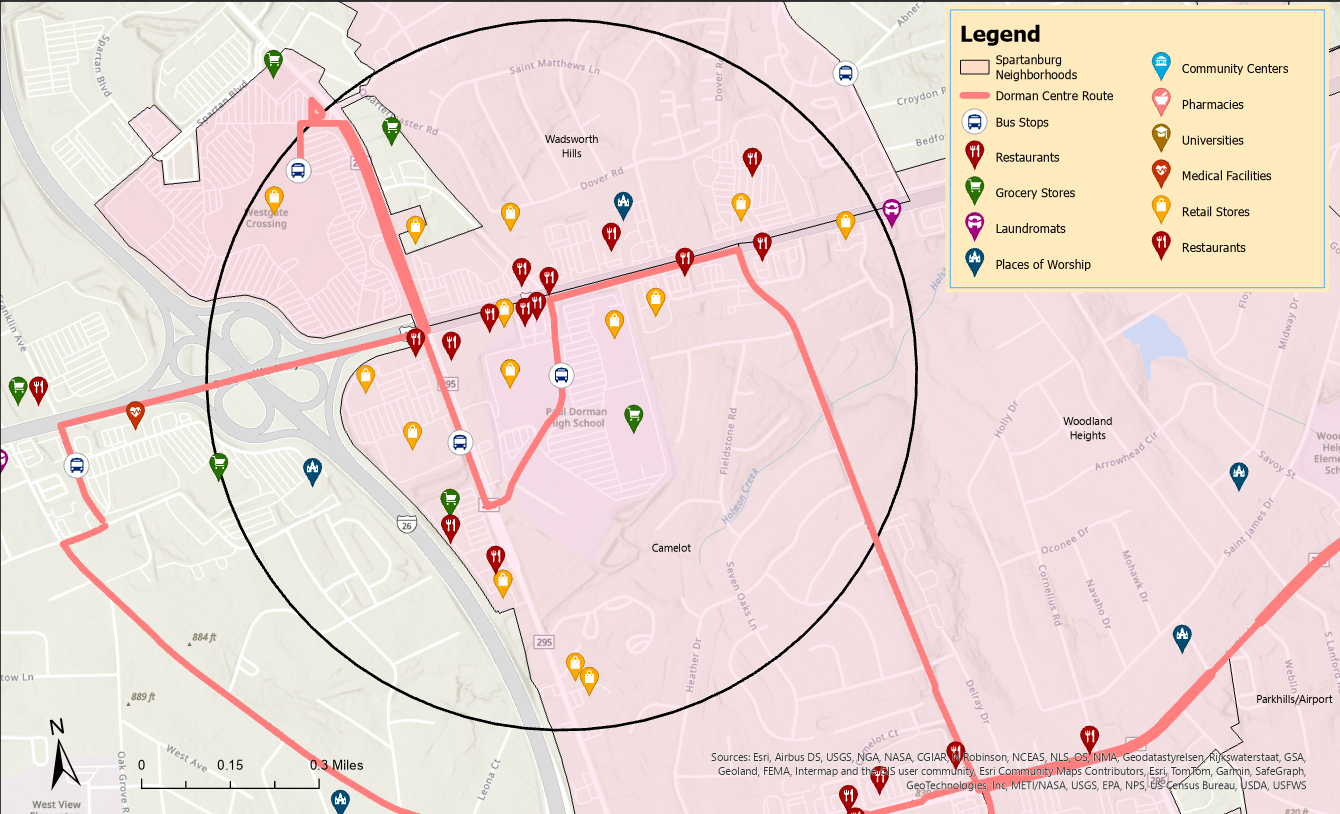
\includegraphics[width=1\linewidth]{dorman center best route.png}
    \caption {Dorman Center Inbound Stop}
    \label{fig:enter-label}
\end{figure}

\begin{figure}[ht]
    \centering
    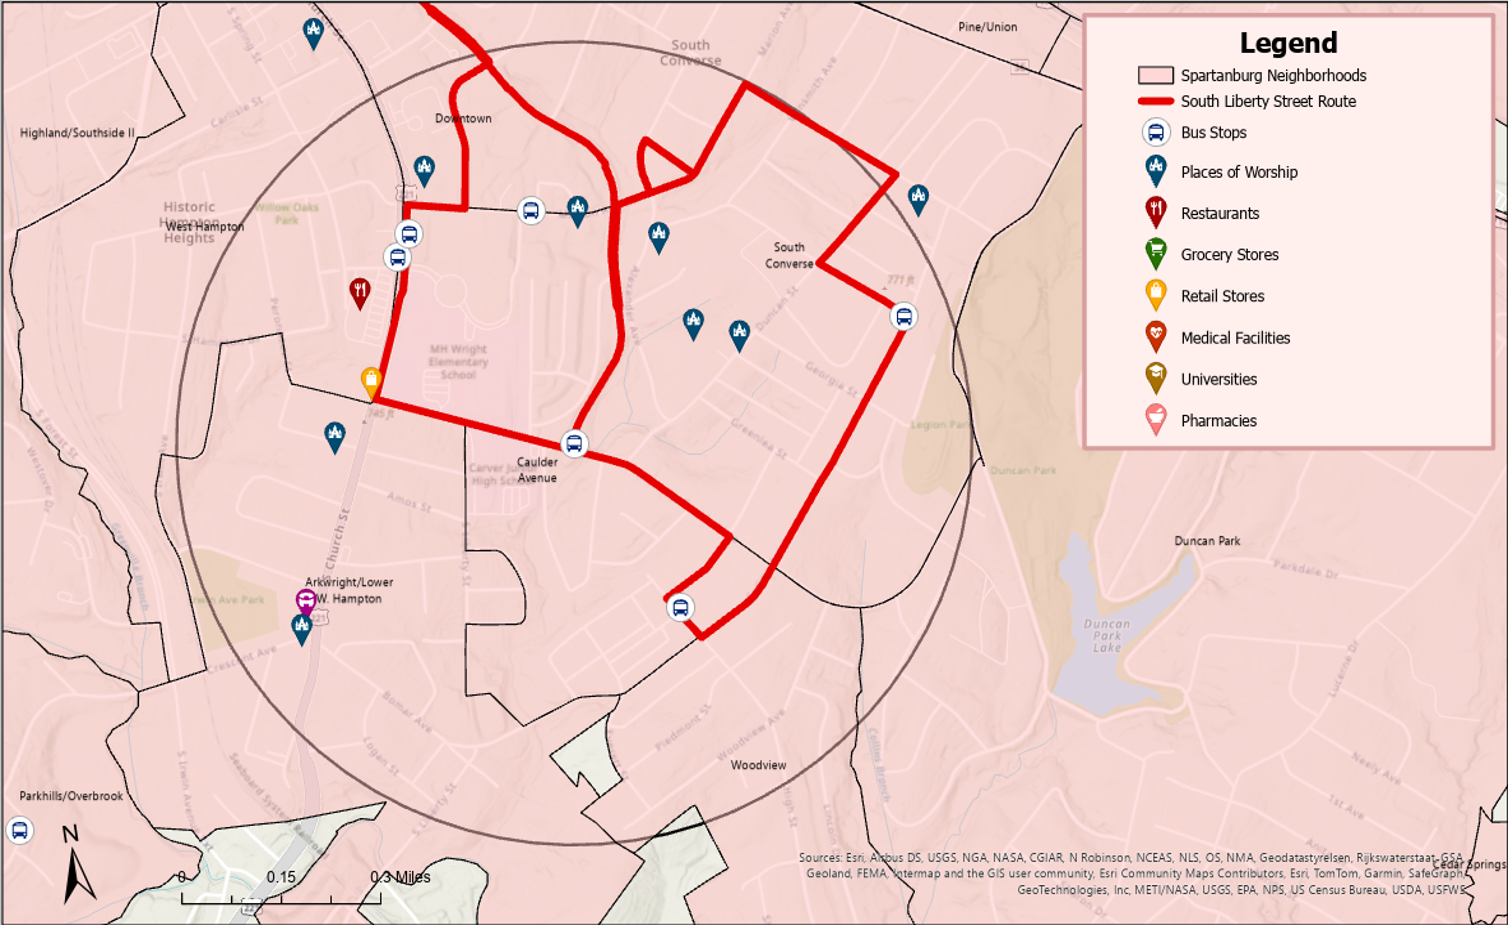
\includegraphics[width=1\linewidth]{libertystop.png}
    \caption {South Liberty Inbound Stop}
    \label{fig:enter-label}
\end{figure}

As previously stated, we were able to fully apply our model to two existing stops in the Spartanburg bus system: Dorman Center Stop 2 Inbound and South Liberty Stop 2 Inbound. The Dorman Center Inbound stop (see Figure 1) is in the center of one of the most dense shopping districts in all of Spartaburg. The 0.6 mile radius around this stop reaches a Walmart Supercenter, several major retail stores such as Ross and Best Buy, as well as part of the local shopping mall.

Within the 0.6 mile radius surrounding this stop, there exists at least one grocery store, three medical facilities, two places of worship, fourteen retail stores, and thirteen restaurants. Plugging this information into our model, we get that this bus stop has an accessibility score P = 10 + 5(3) + 4(2) + 2(14) + 13 = 74. 

The South Liberty Inbound stop (see Figure 2) is in the heart of a large residential district in southern Spartanburg, but still has a considerable amount of important services surrounding it. Within the 0.6 mile radius surrounding this stop, there exists seven places of worship, one laundromat, one retail store, one community center, and one restaurant. Plugging this information into our model, we get that this bus stop has an accessibility score P = 4(7) + 3(1) + 2(1) +2(1) + 1 = 36.

\subsection{Partial Model Application on Four Additional Bus Stops}

We were given additional map data that each have every current bus stop marked, with a corresponding 0.6 mile radius circle drawn around it. Figure 3 has every grocery store in Spartanburg plotted, while Figures 4 and 5 have every pharmacy and medical facility plotted, respectively. Using this data, we were able to apply the limited version of our model to four additional bus stops in the existing system: Crestview Stop 2 Inbound, Hillcrest Stop 2 Outbound, North Church Stop 3 Outbound, and Hillcrest Stop 2 Inbound.

The first two stops that we applied to our simplified model are ones that could be considered average to below average in the context of services and amenities. The Crestview stop lies in a heavily residential district near downtown Spartanburg, and does not have any grocery stores, medical facilities, or pharmacies in the 0.6 mile radius surrounding it. So, though it may provide a solid option for residents to get to the bus, it receives a simplified accessibility score P = 0. The Hillcrest Outbound stop, while lying along a major road that feeds into and out of downtown Spartanburg, is still largely surrounding by residential areas. The 0.6 mile radius around this stop has one grocery store and one medical facility within it, giving a simplified accessibility score P = 10 + 5(1) = 15. 

The latter stops are ones that lie in much denser shopping areas, similarly to the Dorman Center stop. The North Church Outbound stop lies next to a major medical complex as well as several businesses just north of Spartanburg. The 0.6 mile radius around this stop has one grocery store, six medical facilities, and five pharmacies within it. Thus, this stop receives a simplified accessibility score P = 10 + 9 + 5(6) = 49. Lastly, the Hillcrest Inbound stop lies right in the middle of the densest shopping district in eastern Spartanburg. The 0.6 mile radius around this stop has four grocery stores, four pharmacies, and one medical facility within it, giving it a simplified accessibility score P = 10 + 9 + 5(1) = 24.


\begin{figure}
    \centering
    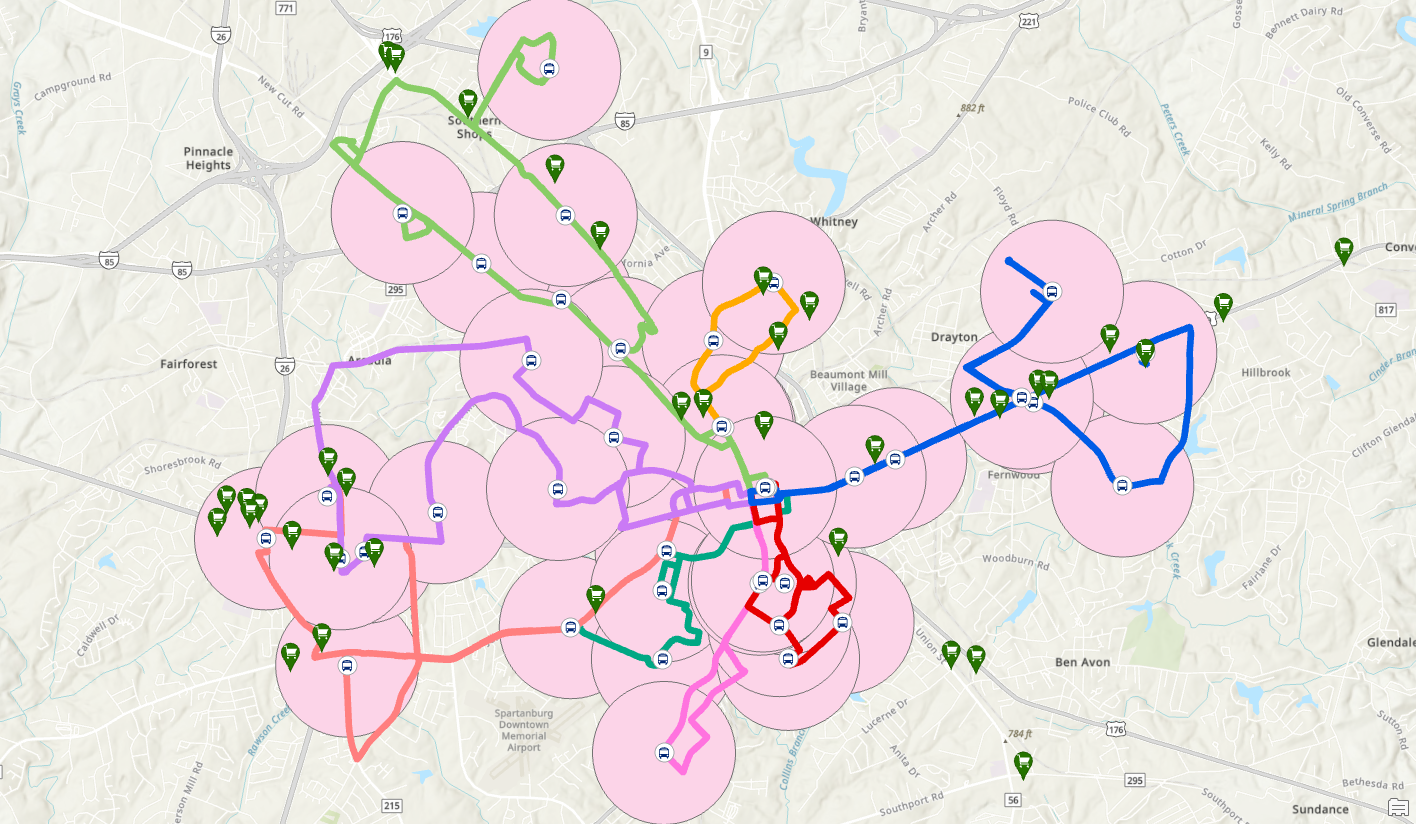
\includegraphics[width=1\linewidth]{groceries_bystop.png}
    \caption{Grocery Stores Along Bus Routes}
    \label{fig:enter-label}
\end{figure}
\begin{figure}
    \centering
    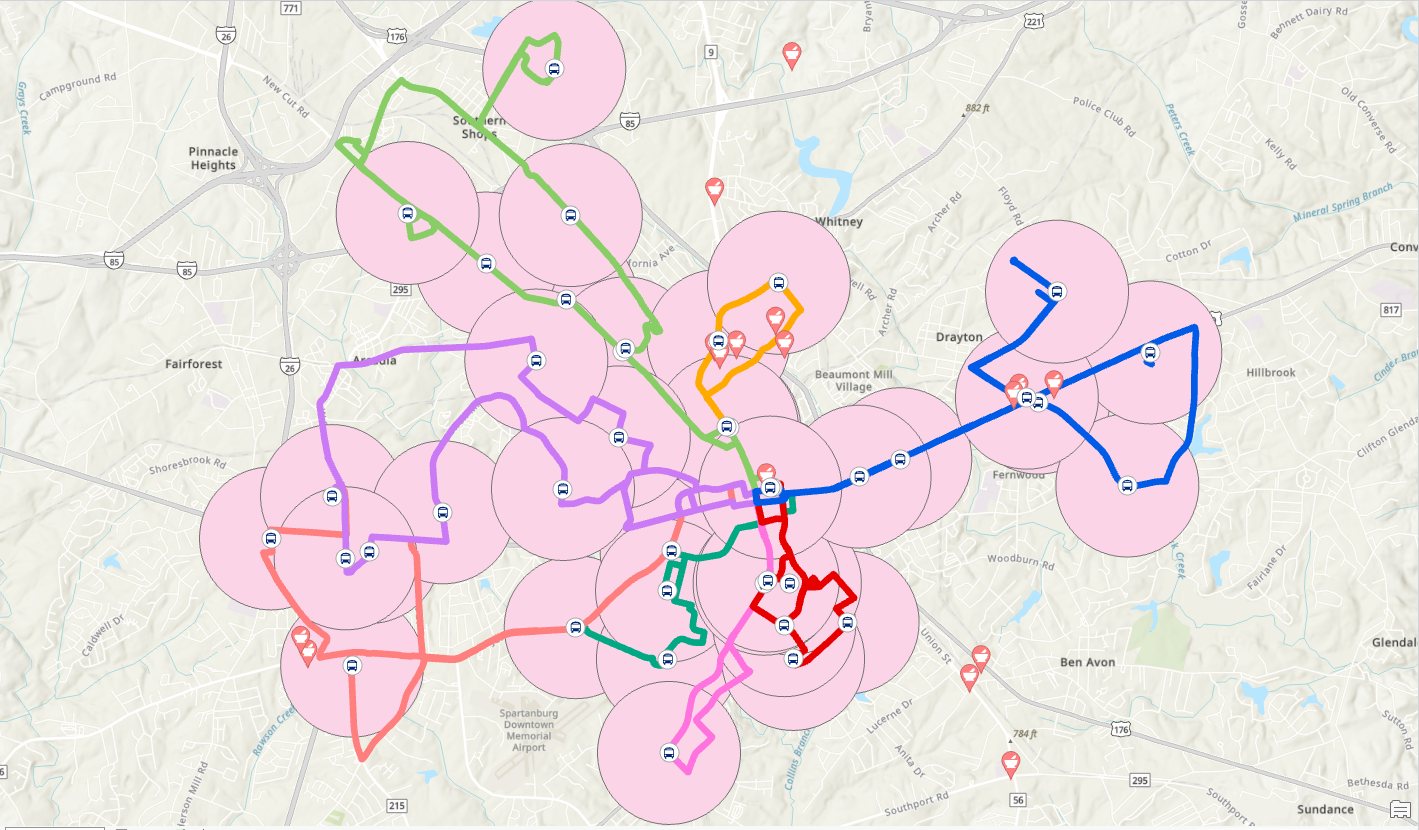
\includegraphics[width=1\linewidth]{pharmacies_bystop.png}
    \caption{Pharmacies Along Bus Routes}
    \label{fig:enter-label}
\end{figure}
\begin{figure}
    \centering
    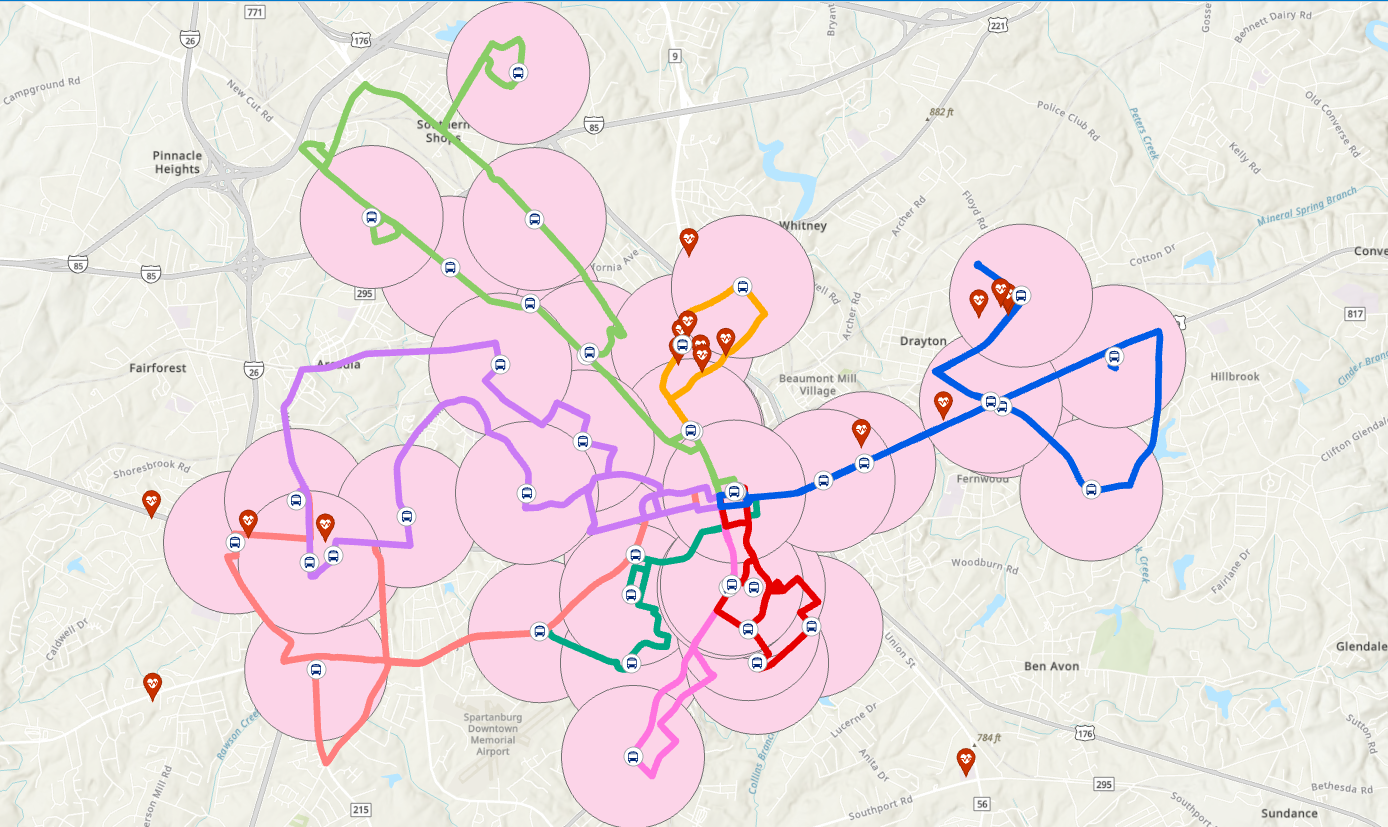
\includegraphics[width=1\linewidth]{medfacilities_bystop.png}
    \caption{Medical Facilities Along Bus Routes}
    \label{fig:enter-label}
\end{figure}


\subsection{General Analysis}

After analyzing our results, we feel that we were able to create a model that accurately assesses accessibility to services and amenities within the Spartanburg community. For the two stops we selected to fully apply our model to, we intentionally picked a heavily commercial stop and a heavily residential stop to see if our model outputted a drastic difference like we would expect. The Dorman Center stop received an accessibility score that is just over double that of the South Liberty stop, which reflects what we were expecting. In addition to this, the residential stops that we evaluated with the simplified model, Crestview and Hillcrest Outbound, received very low scores (0 and 15 respectively). This was expected, as we feel it is much more likely for a heavily residential area to have the smaller, less important services such as laundromats, churches, and restaurants than having the major services and amenities. Conversely, the more dense stops we evaluated, North Church and Hillcrest Inbound, recevied very respectable stores despite the limited amount of services assessed (49 and 24 respectively). In fact, the North Church stop received a higher score than the South Liberty stop, despite only evaluating the top three services for North Church and applying the entire model for South Liberty. We feel that this result further shows that our model appropriately assesses accessibility, by giving high scores to stops with a plentiful amount of services and giving low scores to stops in largely residential areas.



\subsection{Sensitivity Analysis}

We evaluated the accessibility of the bus stops by looking at our three highest-ranking amenities:  grocery stores, pharmacies, and medical facilities.  The same accessibility score weights and radius size surrounding the bus stops were used, with 10 points being given for the presence of at least one grocery store, 9 points for near a pharmacy, and 5 points for each medical facility.  When comparing the Dorman Center stop with the South Liberty stop, the Dorman Center stop’s score is significantly higher than the South Liberty stop.  The Dorman Center, having four grocery stores and three medical facilities earns 25 points from our accessibility score while the South Liberty stop does not contain any of the three services and amenities listed above and has a total of 0 from our accessibility score.  Therefore, examining only these three amenities in comparing Dorman Center stop and the South Liberty stop does not change the ranking of accessibility scores between the two stops.  Because focusing on these three categories does not change the ranking of these two stops based on accessibility scores, it is reasonable to view only these three categories in determining the accessibility scores.  

\section{Conclusions}


The objective of our model was to analyze the existing bus route system in Spartanburg, SC. Using an equation to quantify each service and amenity, we devised a value for each bus stop that would allow us to compare with alternative bus stops. 

Our model did not take into account any residential areas, which is a significant aspect of the model. The residential areas are where the general population lives and will commute to and from the services and amenities. The model did not consider "walk-ability" to and from the bus stops. Things that may decrease the "walk-ability" would be highways and poor sidewalks. The walking speed we devised by an average walking speed of a 65+ year old, which is not entirely inclusive of every passenger of the public transportation. Finally, we did not communicate with the general public of Spartanburg, SC. This would have brought us greater insight into the major necessities of the citizens of the city. 

The further work to be done to this model would be to collaborate with the community. Also, we would recommend compiling a value for each stop and analyzing a median value to create a threshold that would label each stop as "good" or "bad." This would finalize a solution that could be presented to Spartanburg County for further analysis and implementation. 



% -------------------------------------------------------------------
% Bibliography
% -------------------------------------------------------------------


\bibliographystyle{plainnat}
\bibliography{main} 

Alves, F., Cruz, S. S., Ribeiro, A., Silva, A. B., Martins, J. P., \& Cunha, I. (2020). Walkability Index for Elderly Health: A Proposal. \textit{ResearchGate}. https://www.researchgate.net/figure/Walking-average-speed-by-age-group-adapted-from-23-25-52\_tbl2\_344166318. Accessed 2024

Du, J., Qiao, F., \& Yu, L. (2020). Improving Bus Transit Services for Disabled Individuals: Demand Clustering, Bus Assignment, and Route Optimization. \textit{ResearchGate}. https://www.researchgate.net/publication/342728331\_Improving\_Bus\_Transit\_Services\_for\_Disabled\_Individuals\_Demand\_Clustering\_Bus\_Assignment\_and\_Route\_Optimization. Accessed 15 May 2024

Hawas, Y. E., Hassan, M. N., \& Abulibdeh, A. (2016). A multi-criteria approach of assessing public transport accessibility at a strategic level. \textit{Journal of Transport Geography}, \textit{57}, 19–34. doi:10.1016/j.jtrangeo.2016.09.011

Yoo, S., \& Lee, J. (Brian). (2023). Revising bus routes to improve access for the transport disadvantaged: A reinforcement learning approach. \textit{Journal of Public Transportation}, \textit{25}, 100041. doi:10.1016/j.jpubtr.2023.100041

% -------------------------------------------------------------------
% Appendices
% -------------------------------------------------------------------

\newpage

\begin{appendices}
\section{Data Used for Services and Amenities Maps}

This appendix consists of all of the Excel Spreadsheets that we created in order to map data on the services and amenities in Spartanburg. All data was hand-collected through Google Maps and data sets found through websites run by the City of Spartanburg.
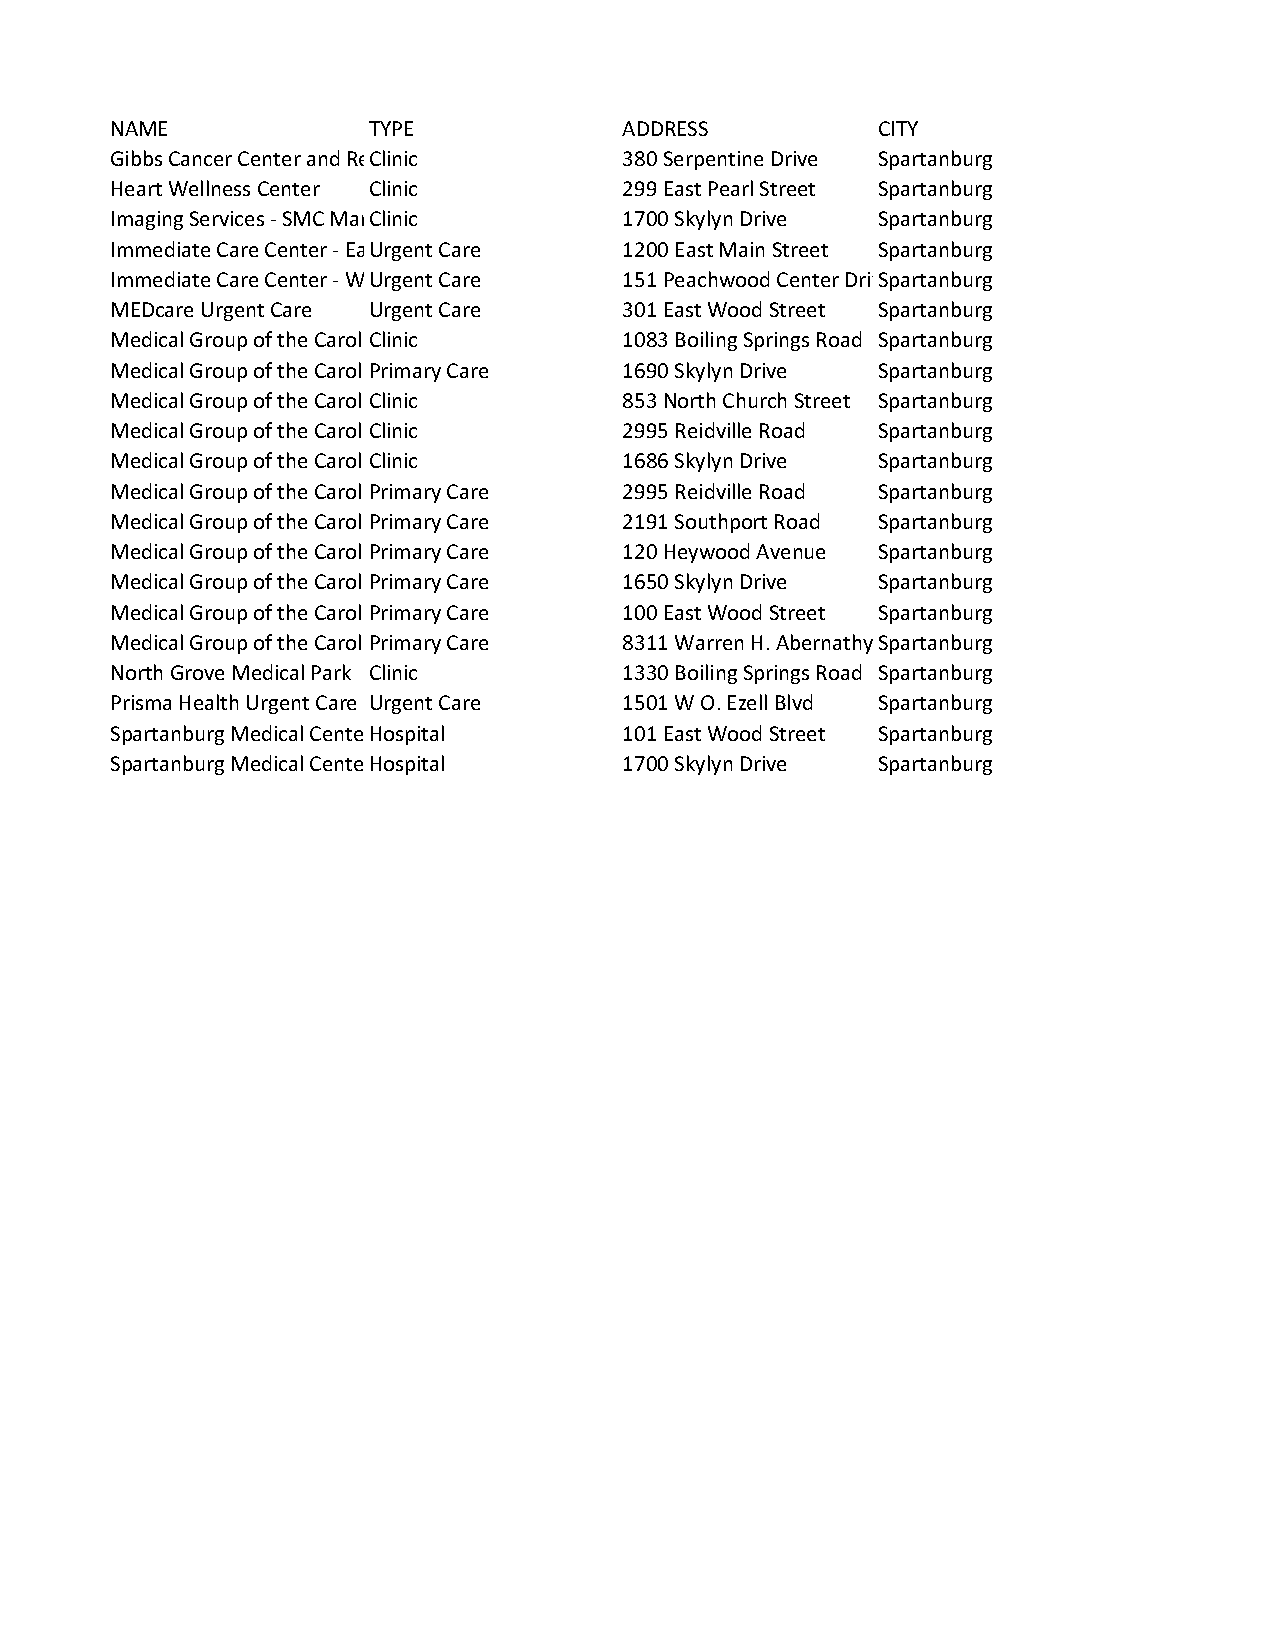
\includepdf[pages=-]{AmenitiesData.pdf}


\section{Data Collected by U.S. Census Bureau on Working Residents of Spartanburg County}

This appendix consists of the spreadsheet we obtained from the U.S. Census Bureau, which provides several summary statistics on the employed residents of Spartanburg County. In this dataset, it shows the amount of vehicles that workers reported as being available to them, as well as showing the means of transportation that workers reported using in order to get to their jobs.

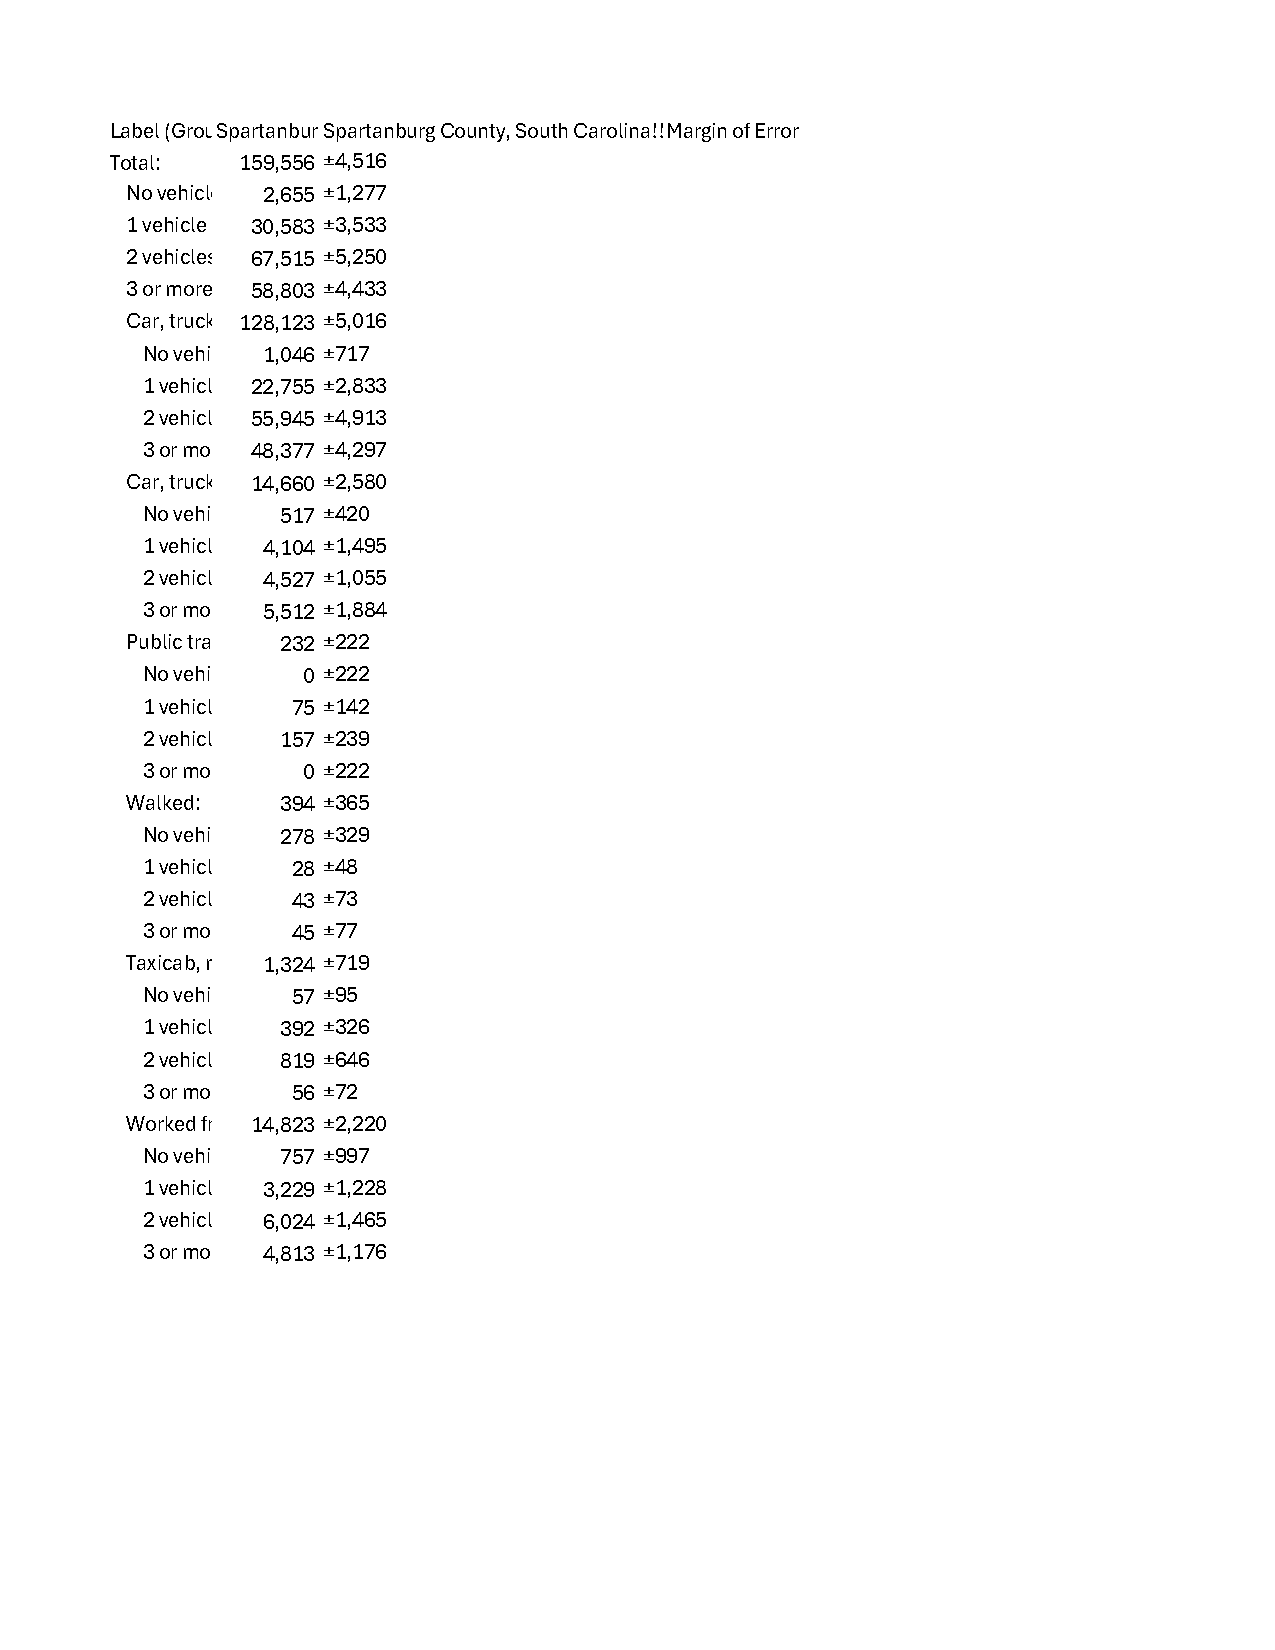
\includepdf[pages=-]{meansoftransportation.pdf}

\section{Data Summary Created for Data in Appendix B}

This appendix consists of a simple data summary that we did using Python programming tools, in order to extract and more deeply analyze the data found in Appendix B.

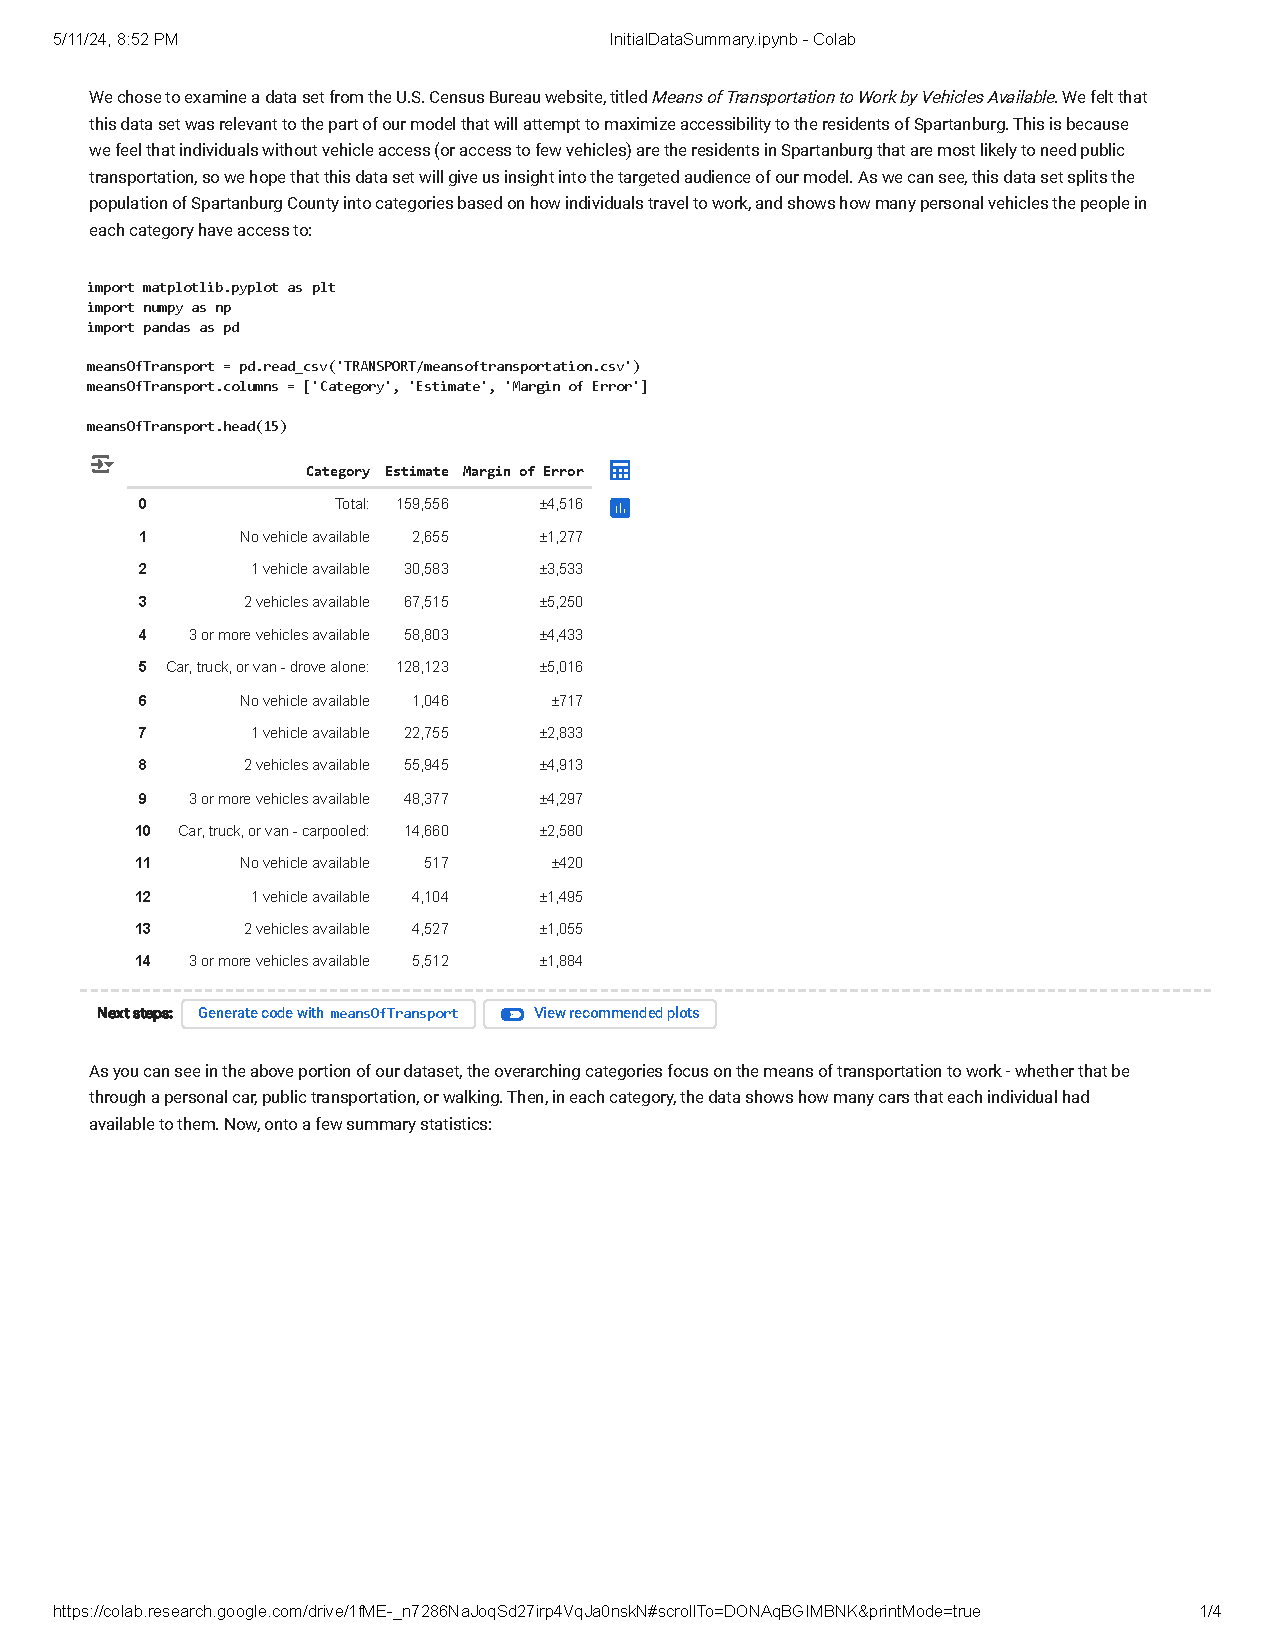
\includepdf[pages=-]{InitialDataSummary.pdf}

\section{Information on Bus Stops}

This appendix consists of a pdf file with the names of all the different bus stops, what routes they are on, and their latitude and longitude location.
\begin{figure}
    \centering
    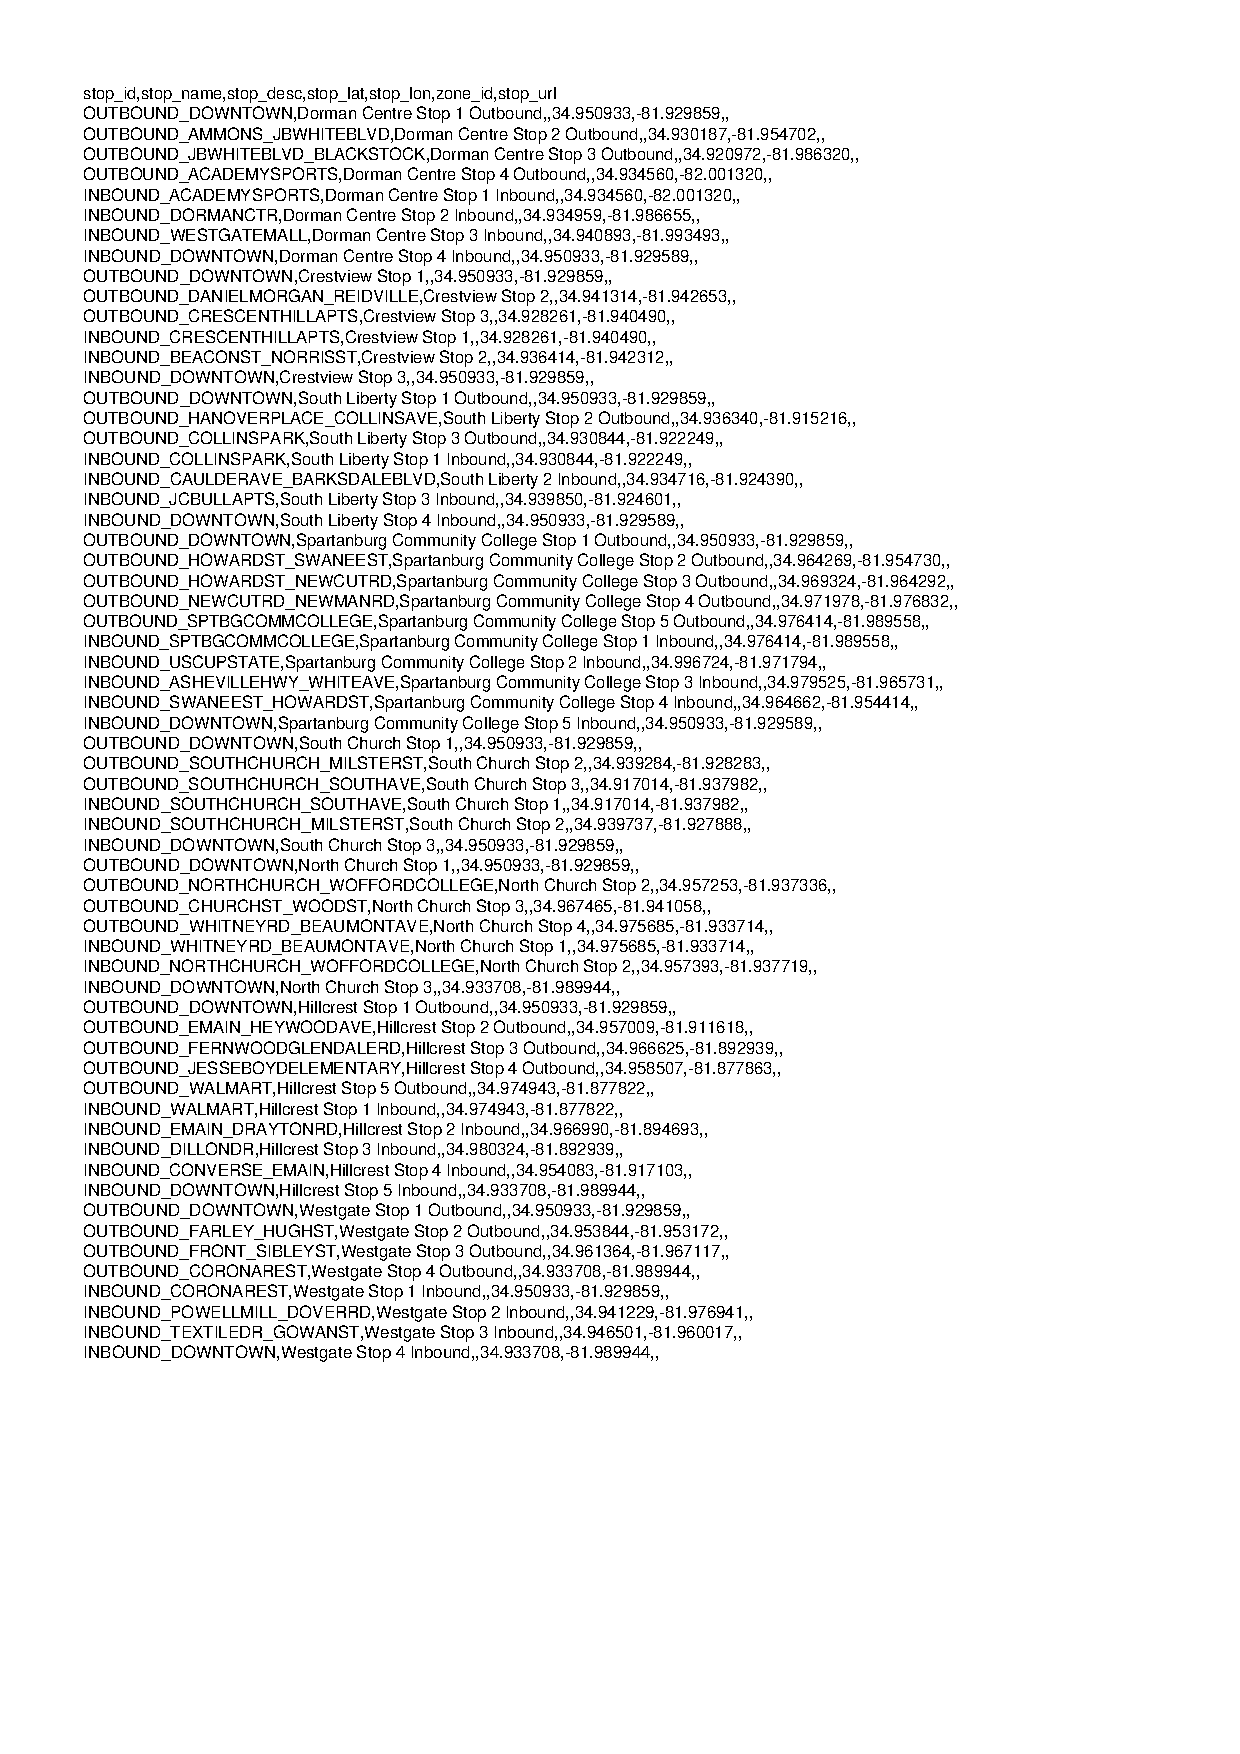
\includegraphics[width=1\linewidth]{GTFS stops.pdf}
\end{figure}
\end{appendices}

\end{document}
